\documentclass{bmcart}

%%%%%%%%%%%%%%%%%%%%%%%%%%%%%%%%%%%%%%%%%%%%%%
%%                                          %%
%% CARGA DE PAQUETES DE LATEX               %%
%%                                          %%
%%%%%%%%%%%%%%%%%%%%%%%%%%%%%%%%%%%%%%%%%%%%%%

%%% Load packages
\usepackage{amsthm,amsmath}
\usepackage{graphicx}
\usepackage{float} % Librería para presentación de imágenes
%\RequirePackage[numbers]{natbib}
\RequirePackage{hyperref}
\usepackage[utf8]{inputenc} %unicode support
%\usepackage[applemac]{inputenc} %applemac support if unicode package fails
%\usepackage[latin1]{inputenc} %UNIX support if unicode package fails

%%%%%%%%%%%%%%%%%%%%%%%%%%%%%%%%%%%%%%%%%%%%%%
%%                                          %%
%% COMIENZO DEL DOCUMENTO                   %%
%%                                          %%
%%%%%%%%%%%%%%%%%%%%%%%%%%%%%%%%%%%%%%%%%%%%%%

\begin{document}

	\begin{frontmatter}
	
		\begin{fmbox}
			\dochead{Research}
			
			%%%%%%%%%%%%%%%%%%%%%%%%%%%%%%%%%%%%%%%%%%%%%%
			%% INTRODUCIR TITULO PROYECTO               %%
			%%%%%%%%%%%%%%%%%%%%%%%%%%%%%%%%%%%%%%%%%%%%%%
			
			\title{Estudio del fenotipo: Discalculia}
			
			%%%%%%%%%%%%%%%%%%%%%%%%%%%%%%%%%%%%%%%%%%%%%%
			%% AUTORES. METER UNA ENTRADA AUTHOR        %%
			%% POR PERSONA                              %%
			%%%%%%%%%%%%%%%%%%%%%%%%%%%%%%%%%%%%%%%%%%%%%%
			
			\author[
			  addressref={aff1},
			  email={ale.pas.mel@uma.es}
			]{\inits{A.P.M.}\fnm{Pascual Mellado} \snm{Alejandro}}
			
			\author[
			  addressref={aff1},
			  email={Acherd@uma.es}
			]{\inits{D.R.A.}\fnm{Ramírez Arco} \snm{David}}
			
			%%%%%%%%%%%%%%%%%%%%%%%%%%%%%%%%%%%%%%%%%%%%%%
			%% AFILIACION. NO TOCAR                     %%
			%%%%%%%%%%%%%%%%%%%%%%%%%%%%%%%%%%%%%%%%%%%%%%
			
			\address[id=aff1]{%                           % unique id
			  \orgdiv{ETSI Informática},             % department, if any
			  \orgname{Universidad de Málaga},          % university, etc
			  \city{Málaga},                              % city
			  \cny{España}                                    % country
			}
		
		\end{fmbox}% comment this for two column layout
		
		\begin{abstractbox}
		
			\begin{abstract} % abstract
			
			%%%%%%%%%%%%%%%%%%%%%%%%%%%%%%%%%%%%%%%%%%%%%%%
			%% RESUMEN BREVE DE NO MAS DE 100 PALABRAS   %%
			%%%%%%%%%%%%%%%%%%%%%%%%%%%%%%%%%%%%%%%%%%%%%%%	
			La discalculia es una condición que dificulta el desarrollo de ciertas habilidades matemáticas, así como  la realización de algunas tareas en las que intervienen operaciones aritméticas. Es similar a la \href{https://hpo.jax.org/app/browse/term/HP:0010522}{dislexia}, fenotipo mas conocido, pero a diferencia de esta,  refleja dificultad en  eventos lógico-matemáticos, sin que con ello se refleje un déficit en las capacidades cognitivas, ni tampoco se presente dificultades con el tiempo, la medición y el razonamiento espacial.
			
			\hfill
			
			En el presente proyecto de investigación procederemos a recolectar información, obteniendo asociaciones de genes y patologías en las que estas mismas proteínas están asociadas.
			
			\end{abstract}
			
			%%%%%%%%%%%%%%%%%%%%%%%%%%%%%%%%%%%%%%%%%%%%%%
			%% PALABRAS CLAVE DEL PROYECTO              %%
			%%%%%%%%%%%%%%%%%%%%%%%%%%%%%%%%%%%%%%%%%%%%%%
			
			\begin{keyword}
			\kwd{Discalculia}
			\kwd{Discapacidad matemática}
			\kwd{Interacción génica}
			\end{keyword}
		
		
		\end{abstractbox}
	
	\end{frontmatter}
	
	%%%%%%%%%%%%%%%%%%%%%%%%%%%%%%%%%
	%% COMIENZO DEL DOCUMENTO REAL %%
	%%%%%%%%%%%%%%%%%%%%%%%%%%%%%%%%%
	
	\section{Introducción}

(Versión Preliminar)

La Discalculia es una discapacidad de aprendizaje específica que afecta la adquisición de habilidades aritméticas. Aunque la falta de  enseñanza, recursos y la baja inteligencia se han relacionado con la etiología de la discalculia, se sabe actualmente que esta discapacidad del aprendizaje es un trastorno cerebral con una predisposición genética familiar \cite{Molko2003}.

\hfill

Las investigaciones se limitaron originalmente a participantes adultos, pero ahora también hay un número creciente de estudios en niños. La investigación en niños con un desarrollo típico indica que la red fronto-parietal está constantemente activa durante el procesamiento de números y la aritmética \cite{originDis}. Ambos muestran similitudes y diferencias con lo que se está observando en adultos. Los niños con discalculia muestran anomalías tanto funcionales como estructurales en esta red.

\hfill


Por otra parte, hay estudios \cite{Molko2003,Shalev2001} que muestran que una forma de este fenotipo está asociado genéticamente con anomalías tanto funcionales como estructurales del surco intraparietal derecho, llevando esta región un papel fundamental en el desarrollo de las habilidades aritméticas.

\hfill

Enfermedades como Alzheimer u otras similares tienen que ver con demencias fronto-temporales \cite{Walterfang2014} que están también fuertemente relacionadas con un número significativo de fenotipos relacionados con los genes implicados en nuestro fenotipo a estudiar

\hfill

El diagnóstico de discalculia generalmente \cite{TreatmentDis} se realiza después de una evaluación exhaustiva, que incluye una revisión del historial del individuo, el desempeño en pruebas estandarizadas y un examen clínico. La evaluación adicional puede incluir una evaluación psico-social para identificar cualquier condición u otros factores que puedan estar contribuyendo a las dificultades matemáticas del individuo.

\hfill

La investigaciones muestran que el tratamiento puede ser eficaz para mejorar el rendimiento matemático en personas con discalculia, con un efecto medio de 0,52 \cite{TreatmentDis} en todos los ensayos de intervención. Es importante que las personas con discalculia reciban el apoyo y las adaptaciones adecuadas para ayudarlos a tener éxito en sus actividades académicas y profesionales.

\hfill

El tratamiento para la discalculia debe adaptarse a las áreas problemáticas específicas del individuo y puede incluir intervenciones  especializadas, tecnología de asistencia y adaptaciones en entornos educativos. Es importante que el tratamiento se inicie temprano \cite{ManagementDis}, preferiblemente en los años de la escuela primaria, y que lo lleven a cabo especialistas capacitados en un entorno individual. Las condiciones comórbidas, como la dislexia, el trastorno por déficit de atención/hiperactividad y otros trastornos mentales, también deben abordarse en el tratamiento.

\hfill



\hfill

\subsection{Información sobre los genes a estudiar}


A continuación se dará una breve información sobre los genes que de mayor grado de interconexión que hemos encontrado al establecer la red del grafo obtenido con String (véase la figura \ref{fig:string1}), un recurso que mas tarde usaremos para los experimentos pero que ahora hemos utilizado a modo informativo para encontrar recursos bibliográficos sobre los genes implicados en nuestro fenotipo

\hfill

\textbf{SQSTM1\cite{SQSTM1}:} Sequestosoma-1; Receptor de autofagia que interactúa directamente tanto con la carga a degradar como con un modificador de autofagia de la familia MAP1 LC3. Puede regular la activación de NFKB1 por TNF-alfa, factor de crecimiento nervioso (NGF) e interleucina-1. Puede desempeñar un papel en la señalización posterior de titina/TTN en las células musculares.

\hfill

\textbf{FUS\cite{FUS}:}Proteína de unión a ARN FUS; Se une tanto al ADN monocatenario como al bicatenario y promueve la hibridación independiente de ATP de los ADN monocatenarios complementarios y la formación del bucle D en el ADN superhelicoidal de doble cadena. Puede desempeñar un papel en el mantenimiento de la integridad genómica; Pertenece a la familia RRM TET.

\hfill

\textbf{VCP\cite{VCP}:} ATPasa del retículo endoplásmico de transición; Necesario para la fragmentación de las pilas de Golgi durante la mitosis y para su reensamblaje después de la mitosis. Participa en la formación del retículo endoplásmico de transición (tER). La transferencia de membranas desde el retículo endoplásmico al aparato de Golgi se produce a través de vesículas de transición de 50-70 nm que se derivan de elementos de transición parcialmente rugosos y parcialmente lisos del retículo endoplásmico (tER). La formación de vesículas en el tER es un proceso dependiente de ATP. El complejo ternario que contiene UFD1, VCP y NPLOC4 se une a proteínas ubiquitinadas.

\hfill

\textbf{CHMP2B\cite{CHMP2B}:}Proteína corporal multivesicular cargada 2b; Probable componente central de la clasificación endosomal requerida para el complejo de transporte III (ESCRT-III) que está involucrado en la formación de cuerpos multivesiculares (MVB) y la clasificación de proteínas de carga endosomal en MVB. Los MVB contienen vesículas intraluminales (ILV) que se generan por invaginación y escisión de la membrana limitante del endosoma y, en su mayoría, se envían a los lisosomas, lo que permite la degradación de las proteínas de la membrana, como los receptores del factor de crecimiento estimulado, las enzimas lisosomales y los lípidos.

\hfill

\textbf{HNRNPA2B1\cite{HNRNPA2B1}:}Ribonucleoproteínas nucleares heterogéneas A2/B1; Ribonucleoproteína nuclear heterogénea (hnRNP) que se asocia con pre-ARNm nacientes y los empaqueta en partículas de hnRNP. La disposición de las partículas de hnRNP en el hnRNA naciente no es aleatoria y depende de la secuencia, y sirve para condensar y estabilizar las transcripciones y minimizar los enredos y los nudos. El empaque juega un papel en varios procesos, como la transcripción, el procesamiento de pre-ARNm, la exportación nuclear de ARN, la ubicación subcelular, la traducción de ARNm y la estabilidad de los ARNm maduros. Forma partículas hnRNP con al menos otras 20 hnRNP diferentes.

\newpage
	\section{Materiales y métodos}

	\section{Resultados}

Se explicaran ahora los resultados que hemos obtenido usando todos los recursos explicados anteriormente:

\subsection{Human Phenotipe Ontology}

\hfill

Tras realizar una búsqueda del fenotipo a investigar, \textit{Dyscalculia}, vemos que se encuentra clasificado como \href{https://hpo.jax.org/app/browse/term/HP:0002442}{HP:0002442} con un total de 13 fenotipos de otras enfermedades asociadas y un total de 24 genes asociados a esta en HPO.

Descargamos un .csv para cargar el listado de genes con sus links en String

\subsection{String}

\hfill

Gracias a las anotaciones en HPO obtenidas del .csv mencionado anteriormente, podemos obtener los genes asociados del fenotipo, y con ello procedemos a la búsqueda de más información acerca de estos utilizando \href{https://string-db.org}{STRING}, una base de datos biológica y un recurso web de interacciones entre proteínas.

\begin{figure}[h]
	\centering
	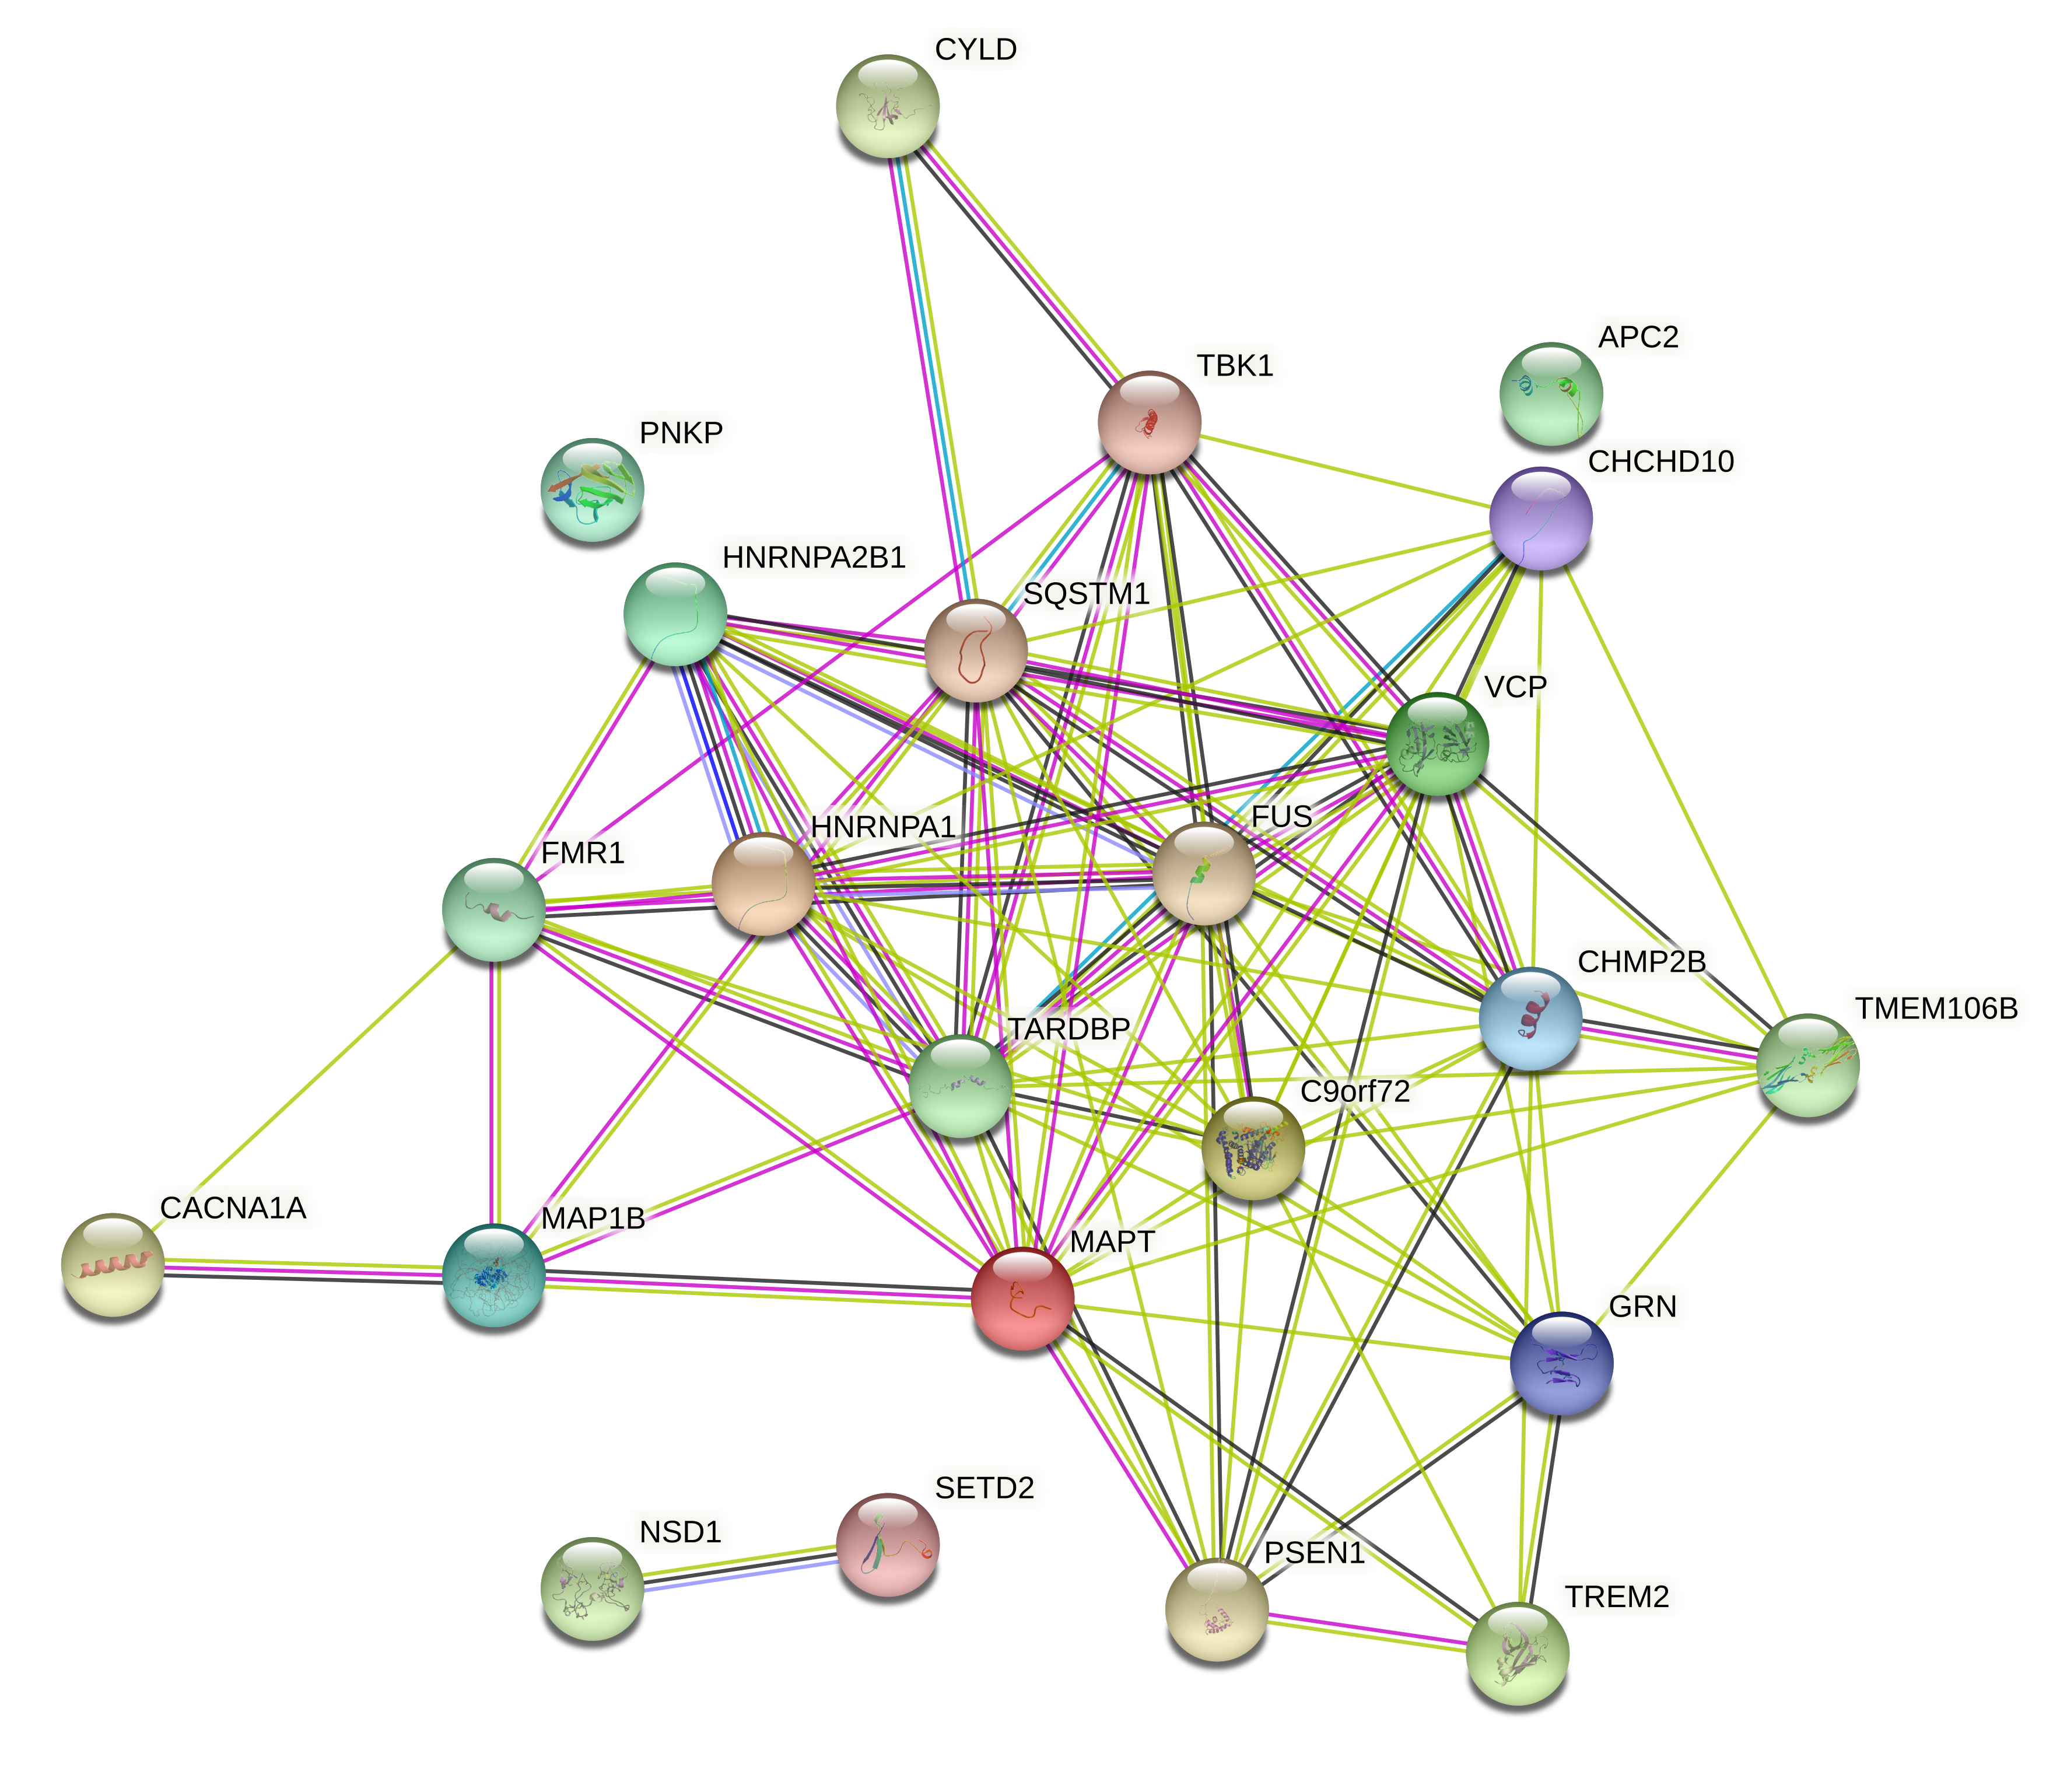
\includegraphics[width=0.90\textwidth]{figures/Gene_Relationship.png}
	\caption{Interacciones proteína-proteína a raíz de los genes relacionados. }
	\label{fig:string1}
\end{figure}

Una vez cargados los genes y sus relaciones en string, procedemos a descargar los ficheros "string-node-degree.tsv" e "string-interactions.tsv".

Se creara también un objeto network de la librería de R stringdb, con las siguientes caracteristicas:

Versión=11
Specie=9606
Score threshold=400

\hfill

Se usara esta network de genes humanos, para buscar genes vecinos de los 24 que teníamos en un principio y realizar una propagación de red con el fin de aumentar el total de genes a estudiar que guarden directa o indirectamente una relación con nuestro fenotipo a estudiar.

\hfill

\subsection{igraph}

Usaremos igraph para convertir nuestro objeto network (genes originalmente relacionados con el  fenotipo mas los genes vecinos de la red general anteriormente citada) en un dataframe que sea procesable por las funciones de clustering para la división en comunidades

\hfill

\subsection{Análisis por comunidades}

Se realizan a continuación los correspondientes pasos para clusterizar nuestro conjunto en distintas comunidades y realizar el correspondiente análisis de enriquecimiento funcional a las adecuadas:

\subsubsection{LinkComm}

Tras una serie de pruebas con distintas funciones de igraph para hacer comunidades, se ha decidido usar la anteriormente citada LinkComm, que nos deja esta imagen como muestra de su trabajo sobre nuestra red de genes: 

\begin{figure}[h]
	\centering
	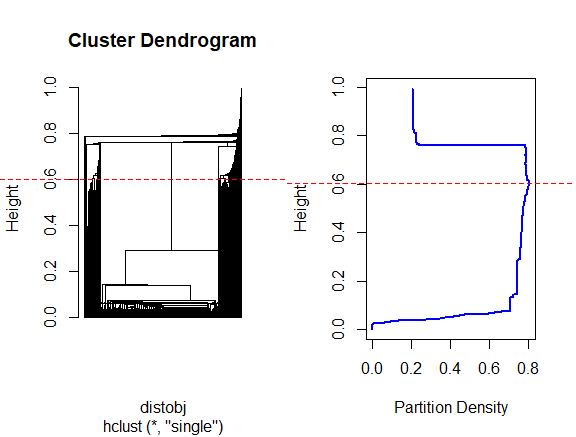
\includegraphics[width=0.90\textwidth]{figures/Grapichs_LinkComm.png}
	\caption{Dendograma del clustering realizado-Relación Altura con Densidad de particion. }
	\label{fig:string1}
\end{figure}

\hfill

\subsubsection{ClusterProfiler}

A continuación se realizara un enriquecimiento funcional con GO (Gene Ontology) para observar las funciones implicadas en la formación de las distintas componentes celulares de las comunidades con un número de genes similar a 20, que supone aproximadamente un 10/100 del total de nuestra red propagada. (En concreto las número 48,71 y 65 que tienen 24,22 y 19 genes respectivamente).

\hfill

Se muestran ahora las principales funciones obtenidas de los tres enriquecimientos:



\hfill

	\newpage

\section{Discusión}

\hfill

A continuación se procede a discutir los resultados que hemos obtenido de las distintas herramientas

\hfill

Tras investigar las distintas interacciones proteína-proteína (véase la figura \ref{fig:string1}) y observar las enfermedades relacionadas con la discalculia en HPO y los distintos artículos científicos citados anteriormente, suponemos la estrecha relación de la discapacidad con un mal funcionamiento del sistema nervioso. En concreto se podría teorizar que existe una relación con las enfermedades de demencia del complejo frontotemporal del cerebro y la esclerosis lateral amiotrófica, pues estas palabras claves aparecen en la mitad de las enfermedades relacionadas con el fenotipo.

\hfill

La demencia de lóbulo frontotemporal, según el estudio \cite{FrontotemoralDementia} es un síndrome clínica y patológicamente heterogéneo, caracterizado por una disminución progresiva del comportamiento o del lenguaje asociado con la degeneración de los lóbulos frontal y temporal anterior. Podemos teorizar que además de con una disminución de las habilidades lingüísticas, esta demencia guarda relación con una disminución de las habilidades aritméticas relacionadas con la discalculia o al menos, los genes implicados en la demencia frontotemporal también son de gran relevancia en la aparición de la discalculia

\hfill

La esclerosis lateral amiotrófica es una enfermedad neurodegenerativa cuyas  pruebas clínicas incluyen signos de daño de las neuronas motoras superior e inferior tanto en las extremidades como en la musculatura bulbar, y en algunos pacientes hay deterioro cognitivo frontotemporal \cite{EsclerosisLateraAmiotrófica}. De nuevo encontramos una relación con el deterioro del lóbulo frontotemporal, en una enfermedad que estaba relacionada a través de muchos de los genes implicados con nuestro fenotipo a estudiar; cada vez se refuerza mas la hipótesis de que nuestro fenotipo esta relacionado con el deterioro del lóbulo frontotemporal

\hfill

A raíz de los artículos recomendados por la base de datos STRING \cite{Walterfang2014,frontotemporal}, suponemos una relación de estos efectos negativos con una mala conexión entre los hemisferios cerebrales, recordemos que el cerebro delega algunas funciones clave como en este caso puede ser la realización de operaciones matemáticas o el reconocimiento numérico y las interconecta a través del Cuerpo Calloso \cite{CorpusCallosum}. Por tanto, un mal funcionamiento de este elemento del sistema puede llevar a una incapacidad de conexión de las funciones de los distintos hemisferios.

\hfill

Observando algunas de las componentes celulares mas relacionas con nuestro conjunto de genes originales (Tabla 1),
encontramos el termino GO “GO:0036464”, este mismo se refiere a la ribonucleoproteina citoplasmática, este tipo de proteína guarda una estrecha relación con los cuerpos GW (cuerpos citoplasmáticos ricos en glicina y triptófano) y tienen funciones altamente especializadas, entre esas funciones se encuentran el transporte neuronal \cite{CytoplasmicRibo}, lo que podría reforzar la hipótesis de que una mala conexión entre ambos hemisferios del cerebro puede originar la discalculia.

\newpage

El segundo termino GO con mas significancia estadística del enriquecimiento a la comunidad de genes original(Tabla 1) , GO:0035770, también se refiere a las ribonucleproteinas, por lo que se puede intuir que los genes que están implicados con nuestro fenotipo también lo están, en menor medida, con las ribonucleoproteinas que anteriormente hemos supuesto que podrían tener relación con el transporte neuronal \cite{CytoplasmicRibo} que reforzaba nuestra hipótesis del fallo de conexión de los hemisferios cerebrales.

\hfill 

Tras un estudio de los análisis de enriquecimiento de las componentes celulares de las tres comunidades que hemos enriquecido (Tabla 2, Tabla 3, Tabla 4), se destaca la presencia del termino GO:0035578, que se corresponde con la componente celular “lumen de gránulo azurófilo”. Parece ser que esta componente celular tienen un papel en la proteína aumentadora de la permeabilidad \cite{Azurophil}, con lo cual un fallo en la formación de esta componente podría llevar a fallos de conexión entre componentes del sistema nervioso.

\hfill

Además se encontró que este tipo de gránulos azurófilos guardan relación los promielocitos neutrófilos de la médula ósea \cite{Azurophil}, lo que reforzaría la relación de los genes vinculados con la discalculia con la enfermedad  esclerosis lateral amiotrófica anteriormente discutida.
	\section{Conclusiones}

\hfill

Remitiéndonos a los resultados y discusiones que hemos obtenido de nuestra investigación sobre la discalculia, podemos concluir que:

\hfill

Los resultados sugieren una posible, en pacientes diagnosticados de discalculia, correlación entre la demencia del lóbulo frontotemporal y el mal funcionamiento entre la interconexión de los hemisferios cerebrales que desemboca en un problema con las capacidades aritmético-lógicas. Un análisis de esa correlación a través de un estadístico en este par de características permitiría una verificación adecuada de esta idea en pacientes con discalculia.

\hfill

Además los resultados siguieren una relación entre los genes responsables de la \textit{esclerosis lateral amiotrófica} y la \textit{discalculia},que a su vez se relaciona con la \textit{demencia del lóbulo frontotemporal}; basándonos en la relación entre este tipo de esclerosis y la demencia del lóbulo frontotemporal, teorizamos que estos tres elementos (demencia del lóbulo frontotemporal, esclerosis lateral amiotrófica y discalculia) forman parte de una red cuya causa-efecto relacionan mecanismos de origen similares, y estos pueden llevar a generar en ciertas circunstancias, una de las patologías u otra.

\hfill

Finalmente, y la vista de nuestras conclusiones, sería interesante realizar estudios en pacientes con discalculia a los que, en un determinado tiempo de estudio, se les proporcionen medicamentos que faciliten la interconexión de los hemisferios cerebrales y el correcto funcionamiento nervioso del lóbulo frontotemporal; y observar si su capacidad aritmético lógica varia con el uso de dichos medicamentos.



	
	
	%%%%%%%%%%%%%%%%%%%%%%%%%%%%%%%%%%%%%%%%%%%%%%
	%% OTRA INFORMACIÓN                         %%
	%%%%%%%%%%%%%%%%%%%%%%%%%%%%%%%%%%%%%%%%%%%%%%
	
	\begin{backmatter}
	
		\section*{Abreviaciones}%% if any
			HPO: Human Phenotype Ontology
			\hfill
			IPP: Interacciones proteína-proteína
			\hfill
			GO: Gene Ontology

		
		\section*{Disponibilidad de datos y materiales}%% if any
			\href{https://github.com/Archerd6/Projecto_Biologia_de_Sistemas}{Proyecto en GitHub}
		
		\section*{Contribución de los autores}
		    
		    A.P.M:  Búsqueda de información sobre los genes a estudiar;
			\hfill
		    
		    D.R.A: Ampliación y cambios en la introducción;
		    \hfill
			
			A.P.M:  Búsqueda de métodos de extracción de información de STRING;
			\hfill
			
			D.R.A: Encargado de la búsqueda bibliográfica científica sobre la discalculia y posibles genes relacionados
			
			\hfill
			
			A.P.M: Encargado del enriquecimiento y la obtención de comunidades
			
			\hfill
			
			D.R.A: Encargado del aspecto técnico y de automatización
		
		
		%%%%%%%%%%%%%%%%%%%%%%%%%%%%%%%%%%%%%%%%%%%%%%%%%%%%%%%%%%%%%%%%%%%%%%%%%%%%%%%%%%%%%%%%
		%% BIBLIOGRAFIA: no teneis que tocar nada, solo sustituir el archivo bibliography.bib %%
		%% por el que hayais generado vosotros                                                %%
		%%%%%%%%%%%%%%%%%%%%%%%%%%%%%%%%%%%%%%%%%%%%%%%%%%%%%%%%%%%%%%%%%%%%%%%%%%%%%%%%%%%%%%%%
		
		\bibliographystyle{bmc-mathphys} % Style BST file (bmc-mathphys, vancouver, spbasic).
		\bibliography{bibliography}      % Bibliography file (usually '*.bib' )
	
	\end{backmatter}
\end{document}
